\documentclass[12pt, a4paper, oneside]{article}\usepackage[]{graphicx}\usepackage[]{color}
%% maxwidth is the original width if it is less than linewidth
%% otherwise use linewidth (to make sure the graphics do not exceed the margin)
\makeatletter
\def\maxwidth{ %
  \ifdim\Gin@nat@width>\linewidth
    \linewidth
  \else
    \Gin@nat@width
  \fi
}
\makeatother

\definecolor{fgcolor}{rgb}{0.345, 0.345, 0.345}
\newcommand{\hlnum}[1]{\textcolor[rgb]{0.686,0.059,0.569}{#1}}%
\newcommand{\hlstr}[1]{\textcolor[rgb]{0.192,0.494,0.8}{#1}}%
\newcommand{\hlcom}[1]{\textcolor[rgb]{0.678,0.584,0.686}{\textit{#1}}}%
\newcommand{\hlopt}[1]{\textcolor[rgb]{0,0,0}{#1}}%
\newcommand{\hlstd}[1]{\textcolor[rgb]{0.345,0.345,0.345}{#1}}%
\newcommand{\hlkwa}[1]{\textcolor[rgb]{0.161,0.373,0.58}{\textbf{#1}}}%
\newcommand{\hlkwb}[1]{\textcolor[rgb]{0.69,0.353,0.396}{#1}}%
\newcommand{\hlkwc}[1]{\textcolor[rgb]{0.333,0.667,0.333}{#1}}%
\newcommand{\hlkwd}[1]{\textcolor[rgb]{0.737,0.353,0.396}{\textbf{#1}}}%

\usepackage{framed}
\makeatletter
\newenvironment{kframe}{%
 \def\at@end@of@kframe{}%
 \ifinner\ifhmode%
  \def\at@end@of@kframe{\end{minipage}}%
  \begin{minipage}{\columnwidth}%
 \fi\fi%
 \def\FrameCommand##1{\hskip\@totalleftmargin \hskip-\fboxsep
 \colorbox{shadecolor}{##1}\hskip-\fboxsep
     % There is no \\@totalrightmargin, so:
     \hskip-\linewidth \hskip-\@totalleftmargin \hskip\columnwidth}%
 \MakeFramed {\advance\hsize-\width
   \@totalleftmargin\z@ \linewidth\hsize
   \@setminipage}}%
 {\par\unskip\endMakeFramed%
 \at@end@of@kframe}
\makeatother

\definecolor{shadecolor}{rgb}{.97, .97, .97}
\definecolor{messagecolor}{rgb}{0, 0, 0}
\definecolor{warningcolor}{rgb}{1, 0, 1}
\definecolor{errorcolor}{rgb}{1, 0, 0}
\newenvironment{knitrout}{}{} % an empty environment to be redefined in TeX

\usepackage{alltt} % Paper size, default font size and one-sided paper
%\graphicspath{{./Figures/}} % Specifies the directory where pictures are stored
%\usepackage[dcucite]{harvard}
\usepackage{rotating}
\usepackage{amsmath}
\usepackage{listings}
\usepackage{setspace}
\usepackage{pdflscape}
\usepackage[flushleft]{threeparttable}
\usepackage{multirow}
\usepackage[comma, sort&compress]{natbib}% Use the natbib reference package - read up on this to edit the reference style; if you want text (e.g. Smith et al., 2012) for the in-text references (instead of numbers), remove 'numbers' 
\usepackage{graphicx}
%\bibliographystyle{plainnat}
\bibliographystyle{agsm}
\usepackage[colorlinks = true, citecolor = blue, linkcolor = blue]{hyperref}
%\hypersetup{urlcolor=blue, colorlinks=true} % Colors hyperlinks in blue - change to black if annoying
%\renewcommand[\harvardurl]{URL: \url}
\IfFileExists{upquote.sty}{\usepackage{upquote}}{}
\begin{document}
\title{R learning notes}
\author{Rob Hayward}
\date{\today}
\maketitle
\section{Apply}
This is from \href{http://blog.datacamp.com/r-tutorial-apply-family/}{R Data Camp}.  This is about manipulating data in a systematic way.  Different functions for different classes. THe aim is to avoid the explicit use of loop. They act on a list, data frame or array and apply a function.  

\lstinline{apply} acts on arrays.  Here it will be applied to a two dimensional array (a matrix). \lstinline{apply(X, Margin, FUN, ...)}. 
\begin{knitrout}
\definecolor{shadecolor}{rgb}{0.969, 0.969, 0.969}\color{fgcolor}\begin{kframe}
\begin{alltt}
\hlstd{x} \hlkwb{<-} \hlkwd{matrix}\hlstd{(}\hlkwd{rnorm}\hlstd{(}\hlnum{30}\hlstd{),} \hlkwc{nrow} \hlstd{=} \hlnum{5}\hlstd{,} \hlkwc{ncol} \hlstd{=} \hlnum{6}\hlstd{)}
\hlkwd{apply}\hlstd{(x,} \hlnum{2}\hlstd{, sum)}
\end{alltt}
\begin{verbatim}
## [1]  4.512017 -1.637159  1.077584  2.308070 -2.174997 -4.154792
\end{verbatim}
\end{kframe}
\end{knitrout}
This will sum the columns (margin = 2).  

\lstinline{lapply} will work on a list, data frame or vector; it returns a list. 

\begin{knitrout}
\definecolor{shadecolor}{rgb}{0.969, 0.969, 0.969}\color{fgcolor}\begin{kframe}
\begin{alltt}
\hlstd{A} \hlkwb{<-} \hlkwd{matrix}\hlstd{(}\hlnum{1}\hlopt{:}\hlnum{9}\hlstd{,} \hlnum{3}\hlstd{,} \hlnum{3}\hlstd{)}
\hlstd{B} \hlkwb{<-} \hlkwd{matrix}\hlstd{(}\hlnum{4}\hlopt{:}\hlnum{15}\hlstd{,} \hlnum{4}\hlstd{,} \hlnum{3}\hlstd{)}
\hlstd{C} \hlkwb{<-} \hlkwd{matrix}\hlstd{(}\hlnum{8}\hlopt{:}\hlnum{10}\hlstd{,} \hlnum{3}\hlstd{,} \hlnum{2}\hlstd{)}
\hlstd{MyList} \hlkwb{<-} \hlkwd{list}\hlstd{(A, B, C)}

\hlcom{# extract the second column from the lists using  the selection operator "["}
\hlkwd{lapply}\hlstd{(MyList,} \hlstr{"["}\hlstd{, ,} \hlnum{2}\hlstd{)}
\end{alltt}
\begin{verbatim}
## [[1]]
## [1] 4 5 6
## 
## [[2]]
## [1]  8  9 10 11
## 
## [[3]]
## [1]  8  9 10
\end{verbatim}
\end{kframe}
\end{knitrout}
The function is the \emph{selection operator}, the next argument is left open so it will take all members of the list, finally the column is selected. 


\section{Lists}
This is from \href{http://rforpublichealth.blogspot.co.uk/2015/03/basics-of-lists.html}{R for Public Health}
The list of a collection of objects
\begin{knitrout}
\definecolor{shadecolor}{rgb}{0.969, 0.969, 0.969}\color{fgcolor}\begin{kframe}
\begin{alltt}
\hlstd{vec} \hlkwb{<-} \hlnum{1}\hlopt{:}\hlnum{4}
\hlstd{df} \hlkwb{<-} \hlkwd{data.frame}\hlstd{(}\hlkwc{y} \hlstd{=} \hlkwd{c}\hlstd{(}\hlnum{1}\hlopt{:}\hlnum{3}\hlstd{),} \hlkwc{x} \hlstd{=} \hlkwd{c}\hlstd{(}\hlstr{"m"}\hlstd{,} \hlstr{"m"}\hlstd{,} \hlstr{"f"}\hlstd{))}
\hlstd{char} \hlkwb{<-} \hlstr{"Hello"}
\hlstd{list1} \hlkwb{<-} \hlkwd{list}\hlstd{(vec, df, char)}
\hlstd{list1}
\end{alltt}
\begin{verbatim}
## [[1]]
## [1] 1 2 3 4
## 
## [[2]]
##   y x
## 1 1 m
## 2 2 m
## 3 3 f
## 
## [[3]]
## [1] "Hello"
\end{verbatim}
\end{kframe}
\end{knitrout}
Any object can be turned into a list with \lstinline{as.list}.  Componets can be named using \lstinline{names} and extraced with the name or with the \lstinline{[[]]}.  If \lstinline{[]} is used, it will return a list not the original class. 
\begin{knitrout}
\definecolor{shadecolor}{rgb}{0.969, 0.969, 0.969}\color{fgcolor}\begin{kframe}
\begin{alltt}
\hlstd{list1[}\hlnum{3}\hlstd{]}
\end{alltt}
\begin{verbatim}
## [[1]]
## [1] "Hello"
\end{verbatim}
\end{kframe}
\end{knitrout}
compared to 
\begin{knitrout}
\definecolor{shadecolor}{rgb}{0.969, 0.969, 0.969}\color{fgcolor}\begin{kframe}
\begin{alltt}
\hlstd{list1[[}\hlnum{3}\hlstd{]]}
\end{alltt}
\begin{verbatim}
## [1] "Hello"
\end{verbatim}
\end{kframe}
\end{knitrout}
Remove lements by assigning them \lstinline{null}.  Convet a list into one  long vector with \lstinline{unlist()}. 

 
\section{Inequality}
This comes from \href{http://freakonometrics.hypotheses.org/18858}{Arthur Charpentier}.  

Not started. 
\begin{knitrout}
\definecolor{shadecolor}{rgb}{0.969, 0.969, 0.969}\color{fgcolor}\begin{kframe}
\begin{alltt}
\hlkwd{library}\hlstd{(}\hlstr{"ineq"}\hlstd{)}
\hlkwd{load}\hlstd{(}\hlkwd{url}\hlstd{(}\hlstr{"http://freakonometrics.free.fr/income_500.RData"}\hlstd{))}
\hlstd{income} \hlkwb{=} \hlkwd{sort}\hlstd{(income)}
\hlstd{income[}\hlnum{1}\hlstd{]}\hlopt{/}\hlkwd{sum}\hlstd{(income)}
\end{alltt}
\begin{verbatim}
## [1] 5.690055e-05
\end{verbatim}
\begin{alltt}
\hlkwd{sum}\hlstd{(income[}\hlnum{1}\hlopt{:}\hlnum{2}\hlstd{])}\hlopt{/}\hlkwd{sum}\hlstd{(income)}
\end{alltt}
\begin{verbatim}
## [1] 0.0001209948
\end{verbatim}
\begin{alltt}
\hlkwd{sum}\hlstd{(income[}\hlnum{1}\hlopt{:}\hlnum{3}\hlstd{])}\hlopt{/}\hlkwd{sum}\hlstd{(income)}
\end{alltt}
\begin{verbatim}
## [1] 0.0002072156
\end{verbatim}
\begin{alltt}
\hlkwd{sum}\hlstd{(income[}\hlnum{1}\hlopt{:}\hlnum{4}\hlstd{])}\hlopt{/}\hlkwd{sum}\hlstd{(income)}
\end{alltt}
\begin{verbatim}
## [1] 0.0003113818
\end{verbatim}
\begin{alltt}
\hlkwd{plot}\hlstd{(}\hlkwd{Lc}\hlstd{(income))}
\end{alltt}
\end{kframe}
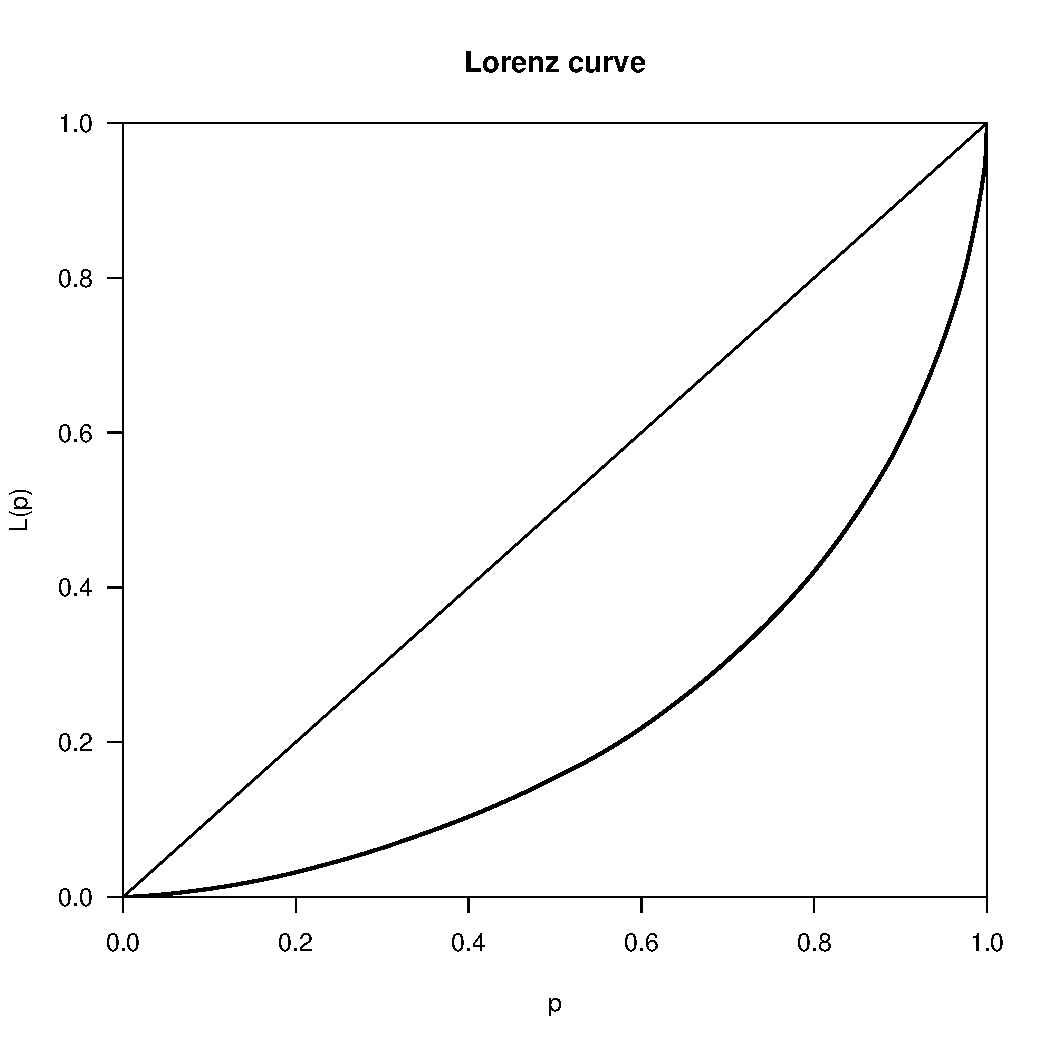
\includegraphics[width=\maxwidth]{figure/library-1} 
\begin{kframe}\begin{alltt}
\hlkwd{points}\hlstd{(}\hlkwd{c}\hlstd{(}\hlnum{0}\hlopt{:}\hlnum{5}\hlstd{)}\hlopt{/}\hlnum{5}\hlstd{,} \hlkwd{c}\hlstd{(}\hlnum{0}\hlstd{,} \hlkwd{cumsum}\hlstd{(income)}\hlopt{/}\hlkwd{sum}\hlstd{(income)),} \hlkwc{pch} \hlstd{=} \hlnum{19}\hlstd{,} \hlkwc{col} \hlstd{=} \hlstr{"blue"}\hlstd{)}
\end{alltt}


{\ttfamily\noindent\bfseries\color{errorcolor}{\#\# Error in xy.coords(x, y): 'x' and 'y' lengths differ}}\end{kframe}
\end{knitrout}
\begin{knitrout}
\definecolor{shadecolor}{rgb}{0.969, 0.969, 0.969}\color{fgcolor}\begin{kframe}
\begin{alltt}
\hlkwd{load}\hlstd{(}\hlkwd{url}\hlstd{(}\hlstr{"http://freakonometrics.free.fr/income_500.RData"}\hlstd{))}
\hlkwd{summary}\hlstd{(income)}
\end{alltt}
\begin{verbatim}
##    Min. 1st Qu.  Median    Mean 3rd Qu.    Max. 
##    2191   23830   42750   77010   87430 2003000
\end{verbatim}
\begin{alltt}
\hlkwd{hist}\hlstd{(}\hlkwd{log}\hlstd{(income),}\hlkwc{probability}\hlstd{=}\hlnum{TRUE}\hlstd{,}\hlkwc{col}\hlstd{=}\hlstr{"light blue"}\hlstd{,}\hlkwc{border}\hlstd{=}\hlstr{"white"}\hlstd{)}
\hlkwd{lines}\hlstd{(}\hlkwd{density}\hlstd{(}\hlkwd{log}\hlstd{(income)),}\hlkwc{col}\hlstd{=}\hlstr{"red"}\hlstd{)}
\hlstd{u}\hlkwb{=}\hlkwd{seq}\hlstd{(}\hlnum{6}\hlstd{,}\hlnum{15}\hlstd{,}\hlkwc{length}\hlstd{=}\hlnum{251}\hlstd{)}
\hlkwd{lines}\hlstd{(u,}\hlkwd{dnorm}\hlstd{(u,}\hlkwd{mean}\hlstd{(}\hlkwd{log}\hlstd{(income)),}\hlkwd{sd}\hlstd{(}\hlkwd{log}\hlstd{(income))),}\hlkwc{col}\hlstd{=}\hlstr{"blue"}\hlstd{)}
\end{alltt}
\end{kframe}
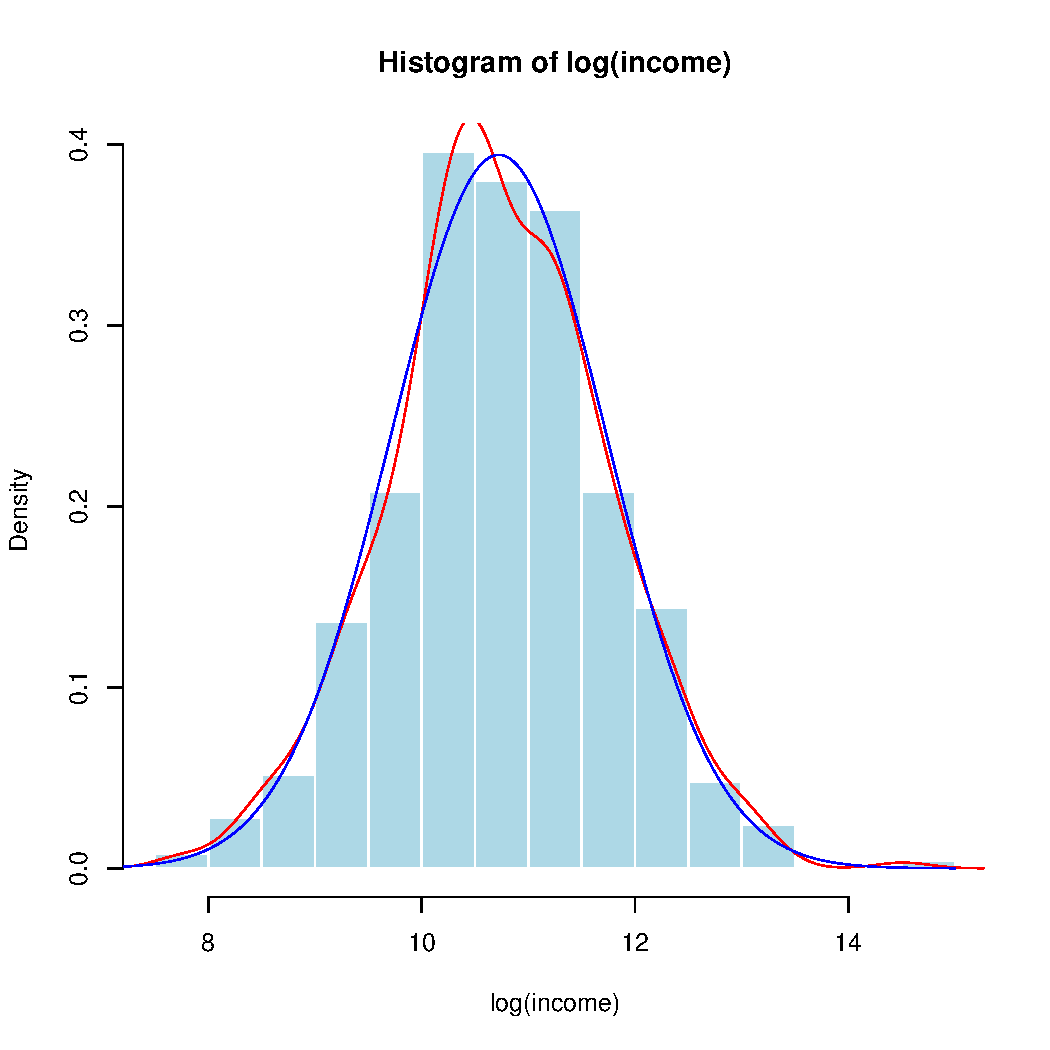
\includegraphics[width=\maxwidth]{figure/da-1} 

\end{knitrout}
These points do not work. The code creates 501 points agaisnt 5. Need to change code.  

\section{Power of tests}
This comes from \href{http://errorstatistics.com/2014/03/12/get-empowered-to-detect-power-howlers/}{Error Statistics Philosophy}.  The statistical stignificance of a test does not mean much without some information on the power of the test. For example, if the smoke alarm is very sensitive, the alarm going off is not a strong indication of a fire; if the alarm is lacking sensitivity, the alarm is a very good signa. 

$H0: \mu \leq 1, \text{against} H1: \mu > 0;$

Let $\sigma = 1, n = 25, \text{so}, (\sigma/\sqrt{n}) = 0.2$

\section{Using dates and time}
This comes from \href{http://www.noamross.net/blog/2014/2/10/using-times-and-dates-in-r---presentation-code.html}{Bonnie Dixon}. This is an overview of using dates and times. 
\begin{knitrout}
\definecolor{shadecolor}{rgb}{0.969, 0.969, 0.969}\color{fgcolor}\begin{kframe}
\begin{alltt}
\hlstd{dt1} \hlkwb{<-} \hlkwd{as.Date}\hlstd{(}\hlstr{"2014-02-15"}\hlstd{)}
\hlstd{dt1}
\end{alltt}
\begin{verbatim}
## [1] "2014-02-15"
\end{verbatim}
\begin{alltt}
\hlstd{dt2} \hlkwb{<-} \hlkwd{as.Date}\hlstd{(}\hlstr{"04/20/2011"}\hlstd{,} \hlkwc{format} \hlstd{=} \hlstr{"%m/%d/%Y"}\hlstd{)}
\hlstd{dt2}
\end{alltt}
\begin{verbatim}
## [1] "2011-04-20"
\end{verbatim}
\begin{alltt}
\hlstd{dt1}\hlopt{-}\hlstd{dt2}
\end{alltt}
\begin{verbatim}
## Time difference of 1032 days
\end{verbatim}
\begin{alltt}
\hlstd{dt2}\hlopt{+}\hlnum{10}
\end{alltt}
\begin{verbatim}
## [1] "2011-04-30"
\end{verbatim}
\end{kframe}
\end{knitrout}
Create a vector of dates and find the difference between them. 
\begin{knitrout}
\definecolor{shadecolor}{rgb}{0.969, 0.969, 0.969}\color{fgcolor}\begin{kframe}
\begin{alltt}
\hlstd{three.dates} \hlkwb{<-} \hlkwd{as.Date}\hlstd{(}\hlkwd{c}\hlstd{(}\hlstr{"2010-07-22"}\hlstd{,} \hlstr{"2011-04-20"}\hlstd{,} \hlstr{"2012-06-10"}\hlstd{))}
\hlstd{three.dates}
\end{alltt}
\begin{verbatim}
## [1] "2010-07-22" "2011-04-20" "2012-06-10"
\end{verbatim}
\begin{alltt}
\hlkwd{diff}\hlstd{(three.dates)}
\end{alltt}
\begin{verbatim}
## Time differences in days
## [1] 272 417
\end{verbatim}
\end{kframe}
\end{knitrout}
Create a sequence of days
\begin{knitrout}
\definecolor{shadecolor}{rgb}{0.969, 0.969, 0.969}\color{fgcolor}\begin{kframe}
\begin{alltt}
\hlstd{six.weeks} \hlkwb{<-} \hlkwd{seq}\hlstd{(dt1,} \hlkwc{length} \hlstd{=} \hlnum{6}\hlstd{,} \hlkwc{by} \hlstd{=} \hlstr{"week"}\hlstd{)}
\hlstd{six.weeks}
\end{alltt}
\begin{verbatim}
## [1] "2014-02-15" "2014-02-22" "2014-03-01" "2014-03-08" "2014-03-15"
## [6] "2014-03-22"
\end{verbatim}
\begin{alltt}
\hlstd{six.weeks} \hlkwb{<-} \hlkwd{seq}\hlstd{(dt1,} \hlkwc{length} \hlstd{=} \hlnum{6}\hlstd{,} \hlkwc{by} \hlstd{=} \hlnum{14}\hlstd{)}
\hlstd{six.weeks}
\end{alltt}
\begin{verbatim}
## [1] "2014-02-15" "2014-03-01" "2014-03-15" "2014-03-29" "2014-04-12"
## [6] "2014-04-26"
\end{verbatim}
\begin{alltt}
\hlstd{six.weeks} \hlkwb{<-} \hlkwd{seq}\hlstd{(dt1,} \hlkwc{length} \hlstd{=} \hlnum{6}\hlstd{,} \hlkwc{by} \hlstd{=} \hlstr{"2 weeks"}\hlstd{)}
\hlstd{six.weeks}
\end{alltt}
\begin{verbatim}
## [1] "2014-02-15" "2014-03-01" "2014-03-15" "2014-03-29" "2014-04-12"
## [6] "2014-04-26"
\end{verbatim}
\end{kframe}
\end{knitrout}
\begin{knitrout}
\definecolor{shadecolor}{rgb}{0.969, 0.969, 0.969}\color{fgcolor}\begin{kframe}
\begin{alltt}
\hlkwd{unclass}\hlstd{(dt1)}
\end{alltt}
\begin{verbatim}
## [1] 16116
\end{verbatim}
\begin{alltt}
\hlstd{dt1}
\end{alltt}
\begin{verbatim}
## [1] "2014-02-15"
\end{verbatim}
\end{kframe}
\end{knitrout}

\subsection{POSIXct}
This is for the use of times. 
\begin{knitrout}
\definecolor{shadecolor}{rgb}{0.969, 0.969, 0.969}\color{fgcolor}\begin{kframe}
\begin{alltt}
\hlstd{tm1} \hlkwb{<-} \hlkwd{as.POSIXct}\hlstd{(}\hlstr{"2009-07-24 23:55:26"}\hlstd{)}
\hlstd{tm1}
\end{alltt}
\begin{verbatim}
## [1] "2009-07-24 23:55:26 BST"
\end{verbatim}
\begin{alltt}
\hlstd{tm2} \hlkwb{<-} \hlkwd{as.POSIXct}\hlstd{(}\hlstr{"25072013 08:32:07"}\hlstd{,} \hlkwc{format} \hlstd{=} \hlstr{"%d%m%Y %H:%M:%S"}\hlstd{)}
\hlstd{tm2}
\end{alltt}
\begin{verbatim}
## [1] "2013-07-25 08:32:07 BST"
\end{verbatim}
\end{kframe}
\end{knitrout}
Specify the time zone
\begin{knitrout}
\definecolor{shadecolor}{rgb}{0.969, 0.969, 0.969}\color{fgcolor}\begin{kframe}
\begin{alltt}
\hlstd{tm3} \hlkwb{<-} \hlkwd{as.POSIXct}\hlstd{(}\hlstr{"2010-12-01 11:42:03"}\hlstd{,} \hlkwc{tz} \hlstd{=} \hlstr{"GMT"}\hlstd{)}
\hlstd{tm3}
\end{alltt}
\begin{verbatim}
## [1] "2010-12-01 11:42:03 GMT"
\end{verbatim}
\end{kframe}
\end{knitrout}
Some calculations with times. 
\begin{knitrout}
\definecolor{shadecolor}{rgb}{0.969, 0.969, 0.969}\color{fgcolor}\begin{kframe}
\begin{alltt}
\hlstd{tm3} \hlopt{>} \hlstd{tm2}
\end{alltt}
\begin{verbatim}
## [1] FALSE
\end{verbatim}
\begin{alltt}
\hlstd{tm1} \hlopt{+} \hlnum{30}
\end{alltt}
\begin{verbatim}
## [1] "2009-07-24 23:55:56 BST"
\end{verbatim}
\begin{alltt}
\hlstd{tm1} \hlopt{-} \hlnum{20}
\end{alltt}
\begin{verbatim}
## [1] "2009-07-24 23:55:06 BST"
\end{verbatim}
\begin{alltt}
\hlstd{tm1} \hlopt{-} \hlstd{tm2}
\end{alltt}
\begin{verbatim}
## Time difference of -1461.359 days
\end{verbatim}
\begin{alltt}
\hlkwd{Sys.time}\hlstd{()}
\end{alltt}
\begin{verbatim}
## [1] "2015-07-30 22:33:12 BST"
\end{verbatim}
\begin{alltt}
\hlkwd{difftime}\hlstd{(tm1,} \hlkwd{as.POSIXct}\hlstd{(}\hlstr{"1970-01-01 00:00:00"}\hlstd{,} \hlkwc{tz} \hlstd{=} \hlstr{"UTC"}\hlstd{,} \hlkwc{units} \hlstd{=} \hlstr{"secs"}\hlstd{))}
\end{alltt}
\begin{verbatim}
## Time difference of 14449.96 days
\end{verbatim}
\end{kframe}
\end{knitrout}
\subsection{POSIXlt}
The 'ct' stands for \emph{calendar time} while 'lt' stands for \emph{local time}.  
\begin{knitrout}
\definecolor{shadecolor}{rgb}{0.969, 0.969, 0.969}\color{fgcolor}\begin{kframe}
\begin{alltt}
\hlstd{tm1.lt} \hlkwb{<-} \hlkwd{as.POSIXlt}\hlstd{(}\hlstr{"2013-07-24 23:55:26"}\hlstd{)}
\hlstd{tm1.lt}
\end{alltt}
\begin{verbatim}
## [1] "2013-07-24 23:55:26 BST"
\end{verbatim}
\begin{alltt}
\hlkwd{unclass}\hlstd{(tm1.lt)}
\end{alltt}
\begin{verbatim}
## $sec
## [1] 26
## 
## $min
## [1] 55
## 
## $hour
## [1] 23
## 
## $mday
## [1] 24
## 
## $mon
## [1] 6
## 
## $year
## [1] 113
## 
## $wday
## [1] 3
## 
## $yday
## [1] 204
## 
## $isdst
## [1] 1
## 
## $zone
## [1] "BST"
## 
## $gmtoff
## [1] NA
\end{verbatim}
\begin{alltt}
\hlkwd{unlist}\hlstd{(tm1.lt)}
\end{alltt}
\begin{verbatim}
##    sec    min   hour   mday    mon   year   wday   yday  isdst   zone 
##   "26"   "55"   "23"   "24"    "6"  "113"    "3"  "204"    "1"  "BST" 
## gmtoff 
##     NA
\end{verbatim}
\end{kframe}
\end{knitrout}
The components of the time object can be extracted. 
\begin{knitrout}
\definecolor{shadecolor}{rgb}{0.969, 0.969, 0.969}\color{fgcolor}\begin{kframe}
\begin{alltt}
\hlstd{tm1.lt}\hlopt{$}\hlstd{sec}
\end{alltt}
\begin{verbatim}
## [1] 26
\end{verbatim}
\begin{alltt}
\hlstd{tm1.lt}\hlopt{$}\hlstd{wday}
\end{alltt}
\begin{verbatim}
## [1] 3
\end{verbatim}
\end{kframe}
\end{knitrout}
Truncate or round off the time. 
\begin{knitrout}
\definecolor{shadecolor}{rgb}{0.969, 0.969, 0.969}\color{fgcolor}\begin{kframe}
\begin{alltt}
\hlkwd{trunc}\hlstd{(tm1.lt,} \hlstr{"days"}\hlstd{)}
\end{alltt}
\begin{verbatim}
## [1] "2013-07-24 BST"
\end{verbatim}
\begin{alltt}
\hlkwd{trunc}\hlstd{(tm1.lt,} \hlstr{"mins"}\hlstd{)}
\end{alltt}
\begin{verbatim}
## [1] "2013-07-24 23:55:00 BST"
\end{verbatim}
\end{kframe}
\end{knitrout}
There is information on the lubridate package in the document referenced. 

\section{Regular Expressions}
This is from the following site \href{http://robinlovelace.net//r/2014/04/14/regex-in-R-RStudio.html}{RobinLovelace}.  The basic regex in R is grep. 

\begin{knitrout}
\definecolor{shadecolor}{rgb}{0.969, 0.969, 0.969}\color{fgcolor}\begin{kframe}
\begin{alltt}
\hlstd{x} \hlkwb{<-} \hlkwd{c}\hlstd{(}\hlstr{"16_24cat"}\hlstd{,} \hlstr{"25_34cat"}\hlstd{,} \hlstr{"35-44catch"}\hlstd{,} \hlstr{"45_54Cat"}\hlstd{,} \hlstr{"55-104fat"}\hlstd{)}
\hlkwd{grep}\hlstd{(}\hlkwc{pattern} \hlstd{=} \hlstr{"cat"}\hlstd{,} \hlkwc{x} \hlstd{= x)}
\end{alltt}
\begin{verbatim}
## [1] 1 2 3
\end{verbatim}
\end{kframe}
\end{knitrout}
Note the way that any case of the pattern is identified but it must be the correct case. 
\begin{knitrout}
\definecolor{shadecolor}{rgb}{0.969, 0.969, 0.969}\color{fgcolor}\begin{kframe}
\begin{alltt}
\hlstd{x} \hlkwb{<-} \hlkwd{c}\hlstd{(}\hlstr{"16_24cat"}\hlstd{,} \hlstr{"25_34cat"}\hlstd{,} \hlstr{"35_44catch"}\hlstd{,} \hlstr{"45_54Cat"}\hlstd{,} \hlstr{"55-104fat"}\hlstd{)}
\hlkwd{grep}\hlstd{(}\hlkwc{pattern} \hlstd{=} \hlstr{"cat"}\hlstd{,} \hlkwc{x} \hlstd{= x,}\hlkwc{ignore.case} \hlstd{= T)}
\end{alltt}
\begin{verbatim}
## [1] 1 2 3 4
\end{verbatim}
\end{kframe}
\end{knitrout}
The function grepl is the same as grep but the output is a logical value.

The fu8nction strsplit will split a string. In this case around the underscore.
\begin{knitrout}
\definecolor{shadecolor}{rgb}{0.969, 0.969, 0.969}\color{fgcolor}\begin{kframe}
\begin{alltt}
\hlkwd{strsplit}\hlstd{(x,} \hlkwc{split} \hlstd{=} \hlstr{"_"}\hlstd{)}
\end{alltt}
\begin{verbatim}
## [[1]]
## [1] "16"    "24cat"
## 
## [[2]]
## [1] "25"    "34cat"
## 
## [[3]]
## [1] "35"      "44catch"
## 
## [[4]]
## [1] "45"    "54Cat"
## 
## [[5]]
## [1] "55-104fat"
\end{verbatim}
\end{kframe}
\end{knitrout}
To return the second element, 
\begin{knitrout}
\definecolor{shadecolor}{rgb}{0.969, 0.969, 0.969}\color{fgcolor}\begin{kframe}
\begin{alltt}
\hlkwd{library}\hlstd{(stringr)}
\hlkwd{str_split_fixed}\hlstd{(x,} \hlstr{"_"}\hlstd{,} \hlnum{2}\hlstd{)[,}\hlnum{2}\hlstd{]}
\end{alltt}
\begin{verbatim}
## [1] "24cat"   "34cat"   "44catch" "54Cat"   ""
\end{verbatim}
\end{kframe}
\end{knitrout}
For finding and replacing, use sub for the first case and gsub for all cases. 
\begin{knitrout}
\definecolor{shadecolor}{rgb}{0.969, 0.969, 0.969}\color{fgcolor}\begin{kframe}
\begin{alltt}
\hlkwd{gsub}\hlstd{(}\hlkwc{pattern} \hlstd{=} \hlstr{"cat$"}\hlstd{,} \hlkwc{replacement} \hlstd{=} \hlstr{"fat"}\hlstd{,} \hlkwc{x} \hlstd{= x,} \hlkwc{ignore.case} \hlstd{= T)}
\end{alltt}
\begin{verbatim}
## [1] "16_24fat"   "25_34fat"   "35_44catch" "45_54fat"   "55-104fat"
\end{verbatim}
\end{kframe}
\end{knitrout}
To insert an additional letter in all cases where there are two numbers followed by a letter, but only when the first number is 3 or less, 
\begin{knitrout}
\definecolor{shadecolor}{rgb}{0.969, 0.969, 0.969}\color{fgcolor}\begin{kframe}
\begin{alltt}
\hlkwd{gsub}\hlstd{(}\hlstr{"([1-3][1-9][a-z])"}\hlstd{,} \hlstr{"m\textbackslash{}\textbackslash{}1"}\hlstd{, x,} \hlkwc{perl} \hlstd{= T, )}
\end{alltt}
\begin{verbatim}
## [1] "16_m24cat"  "25_m34cat"  "35_44catch" "45_54Cat"   "55-104fat"
\end{verbatim}
\end{kframe}
\end{knitrout}



\end{document}
